% !TEX encoding = UTF-8 Unicode
% !TEX root = ../../../Masterthesis.tex
\section{Main Title}\label{sec:STTMP Main Title}
%-----------------------------------------------------------------------------
% Intro
%-----------------------------------------------------------------------------
\begin{figure}[h!]
\center
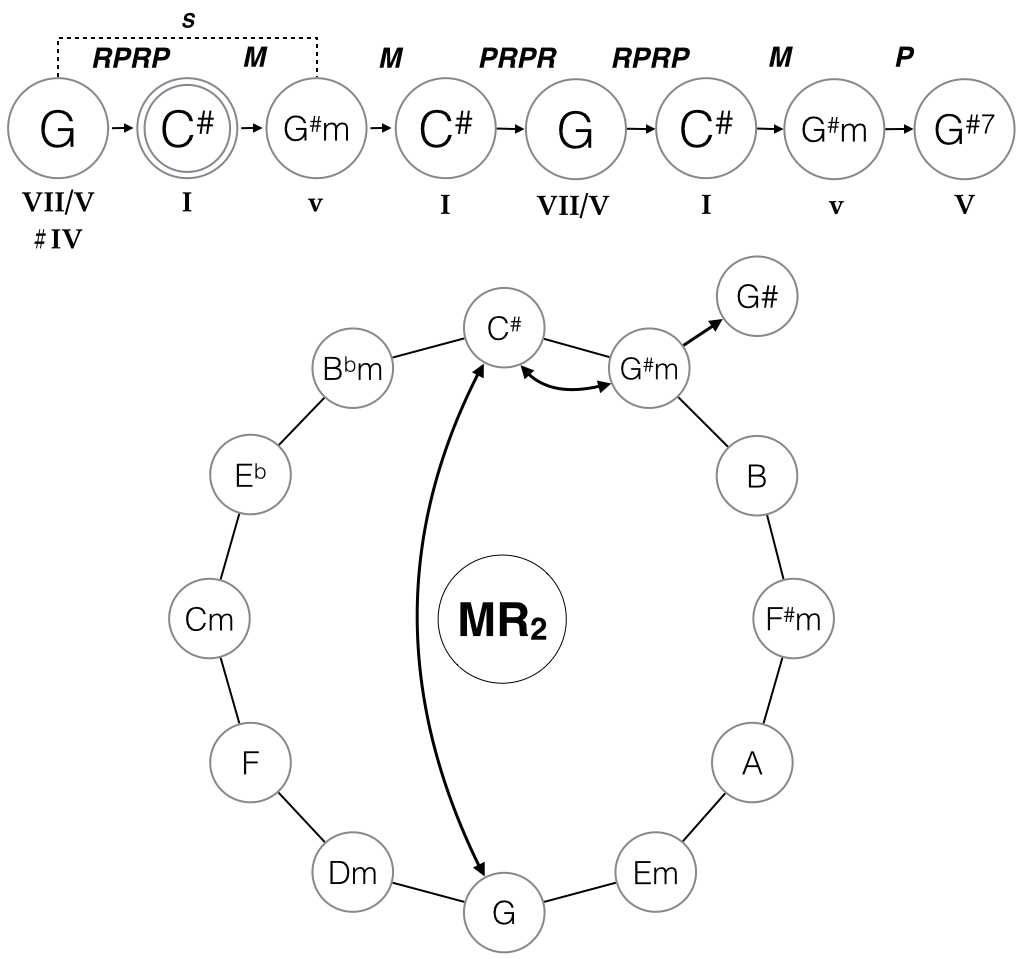
\includegraphics[width=\linewidth]{STTMP_Main_Title_intro}
	\caption{ST:TMP: Main Title Intro}
	\label{fg:sttmp_main_title_intro}
	\setfloatalignment{b}
\end{figure}
\noindent The music starts with the Paramount logo, and music is played with the opening credits. The form is reminiscent of a Rondo, where the overall structure is ABABA, containing development parts.
In figure \ref{fg:sttmp_main_title_intro}, we see that the first two chords in this main title tell us quite a few things. First of all, the relation between them are a tritone, and the G does not seem to be the tonic. The \acf{MTTP} in science fiction movies have been around since the 1950's\shortcite{murphy_major_2006} and the origins of tritone progression related to something extraterrestrial is generally believed to stem from Holst's: The Planets,\footnote{Mars: Strings play col legno in 5/8, while the brass plays the main motif: [0,7,6]  bringing the tritone into play as the harbinger of death; Mars, the God of War.} thus signifying both the monstrous\shortcite{fairweather_jerry_2014} and outer space. By executing this from the very beginning, he implicitly states that this tale will not necessarily happen on earth and, at the very least, contains imagery depicting something outer-wordly, i.e. there will be a monster in some form or another. 

The G in this progression poses a challenge to traditional tonal thinking, and if one assumes G as tonic the rest that follows is, at best, very unstable. The \ciss seems to carry the majority of tonic weight. The G in the context of \ciss could be interpreted as either \(\sharp{IV}\) or \(VII/V\) but both cloud the musical intention. \gissm could be considered a mixolydian \(v\) thus making a \textbf{S} relationship with G. The cadence is, thanks to the \giss, acting as a \(({\flat}VII)\) subtonic cadence to \bflat giving a nod to the musical practices in established in Western's between 1920 and 1940.\marginnote[-2cm]{Frank Lehman's essay on ''Hollywood Cadences'' tells us this type of cadence is common with the practices found in Westerns and its sub-genres. This provides a clue to what we can expect. Roddenberry himself has called Star Trek a ''space western'' and the cadences used are evidence of this:  ''The cadence€™s capacity to index film genre is as potent as its ability to punctuate and structure dramatic action.''(\citealt{lehman_hollywood_2013})}

%-----------------------------------------------------------------------------
% A and A' 
%-----------------------------------------------------------------------------
Figure \ref{fg:sttmp_main_title_a}, A shows that the main theme is situated harmonically around fifths. The tonality is clearly mixolydian with evidence enclosed in the minor \(v\). The sublime references to ''cowboy music'' keeps recurring with the oscillating \(I \Leftrightarrow \flat{VII}\). The part repeats and ends on F. I have also provided a simple \textit{Tonnetz} graph\footnote{Blue is minor and Red is major.} of the passage to show that it is possible to discern a pattern using this. It is, however, not something I will continue to use as is to obscure in its reading. 

\begin{figure*}
\center
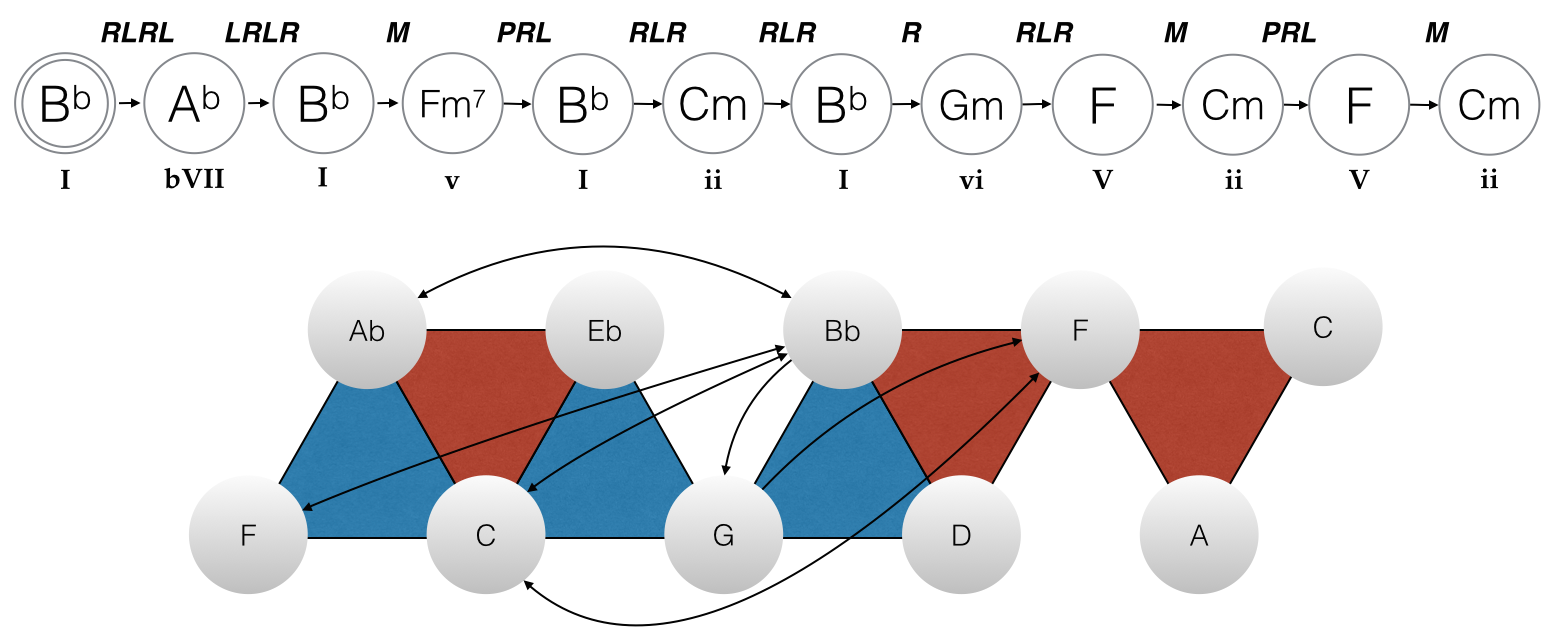
\includegraphics[width=\linewidth]{STTMP_Main_Title_A}
	\caption{ST:TMP: Main Title A}
	\label{fg:sttmp_main_title_a}
\end{figure*}


%-----------------------------------------------------------------------------
% B and B'
%-----------------------------------------------------------------------------
\begin{figure}[h!]
\center
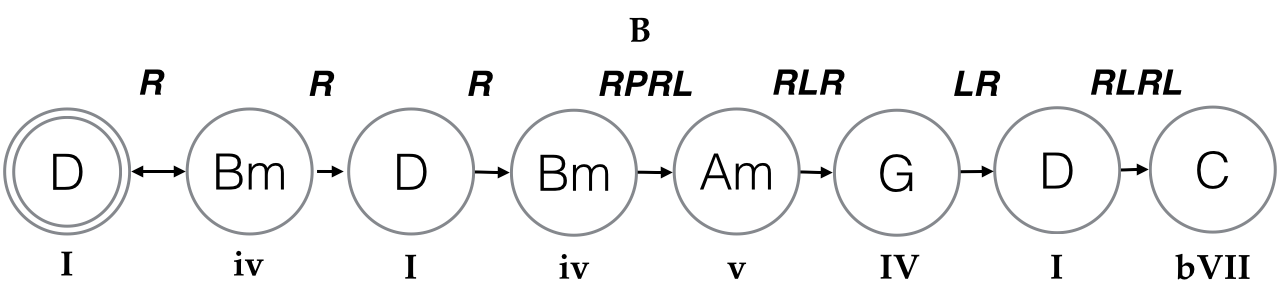
\includegraphics[width=\linewidth]{STTMP_Main_Title_B}
	\caption{ST:TMP Main Title B}
	\label{fg:sttmp_main_title_b}
	\setfloatalignment{b}
\end{figure}

The entrance to B, figure \ref{fg:sttmp_main_title_b}, is via F, which acts as (\(\flat{III}\)) in the new tonic making it a \textit{type 2} flat mediant modulation\shortcite{lehman_hollywood_2013} seen both from the tonic D and F. The music is still saturated in mixolydian scale, providing both the minor \(v\) and the \(bVII\).

\begin{figure}[h!]
\center
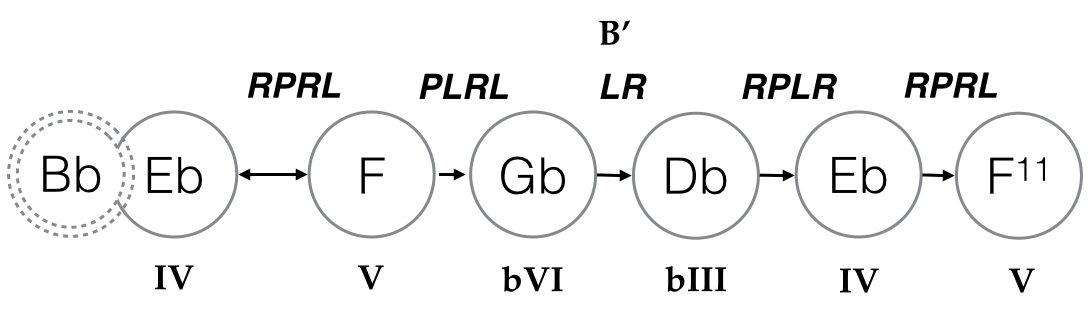
\includegraphics[width=\linewidth]{STTMP_Main_Title_B'_1}
	\caption{ST:TMP: Main Title B' 1}
	\label{fg:sttmp_main_title_b_1}
	\setfloatalignment{b}
\end{figure}

B' starts with the modulation from the previous C/D  to \eflat. The C/D, in this case, acts as bVII in D, but if one would think it as a \textbf{Dominant} in G: D\(^{11}\), in relation to \eflat it provides a \textit{deceptive cadence}, making the formula: \(V(D^{11})\Rightarrow{\flat}VI(E{\flat})\). But the tonal trickery does not stop there. Goldsmith makes \eflat to be \(IV\), making the key \bflat. The evidence for that lies in the cascading cadences that follow. If F is \(V\) then its connections to the other chords can be seen in figure \ref{fg:sttmp_main_title_b_cadence}. Every one of those connections seen individually and in relation to F is tried and true. What is unusual, is that instead of doing one of them, Goldsmith unleashes a string of them, making a circular modulating network.

\begin{figure}[h!]
\center
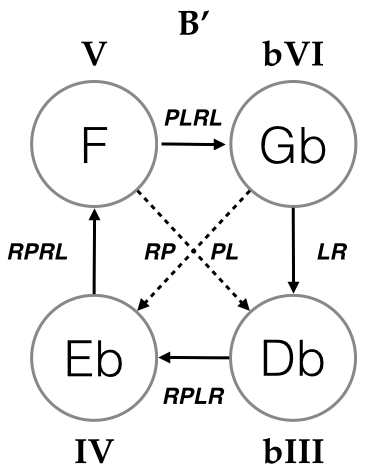
\includegraphics[width=0.4\linewidth]{STTMP_Main_Title_B'_2}
	\caption{ST:TMP: Main Title B' cadence}
	\label{fg:sttmp_main_title_b_cadence}
\end{figure}



%-----------------------------------------------------------------------------
% A''
%-----------------------------------------------------------------------------
\begin{figure}[h!]
\center
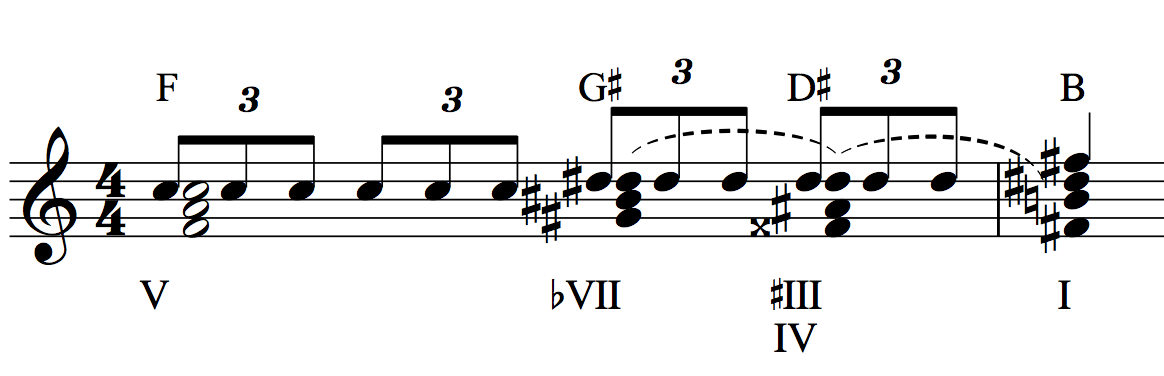
\includegraphics[width=\linewidth]{STTMP_Main_Title_A''}
	\caption{ST:TMP: Main Title A'' cadence}
	\label{fg:sttmp_main_title_a''_cadence}
	\setfloatalignment{b}
\end{figure}

So far the overall structure has been: Intro, A, A', B, B' and now A returns mostly identically to previous iterations, breaking the mold with only one repetition (figure \ref{fg:sttmp_main_title_a''_cadence}).The modulation in m.24 works through three chords sharing one common tone, thus making the maximal usage of one tone to serve as a modulation catalyst, \giss: \(\hat{5}\), \diss: \(\hat{1}\) and B: \(\hat{3}\). Even though the key is \bflat, the relation between F and B is a \ac{MTTP}, further solidifying its position in the Star Trek universe. 

%-----------------------------------------------------------------------------
% B''
%-----------------------------------------------------------------------------
\begin{figure}[h!]
\center
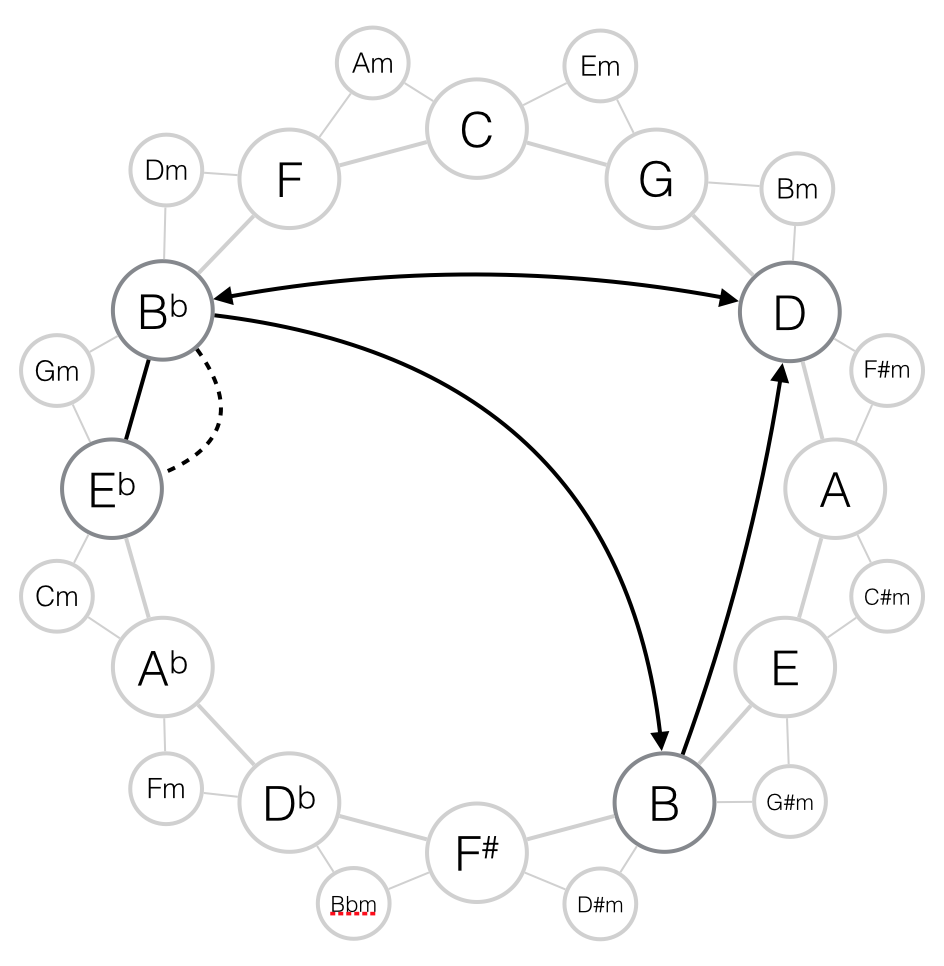
\includegraphics[width=0.7\linewidth]{STTMP_Main_Title_AB_modulation_chart}
	\caption{ST:TMP: Main Title AB modulation chart}
	\label{STTMP_Main_Title_AB_modulation_chart}
	\setfloatalignment{b}
\end{figure}

With the reintroduction of B'', we see that the melody is slightly more relaxed and the modulation formula has changed. When looking at figure \ref{STTMP_Main_Title_AB_modulation_chart} one sees that the modulation described in \ref{fg:sttmp_main_title_a''_cadence} has carried the tonal center further away from \bflat than in previous modulations. The transition from B'' to B''' also follows a different formula; instead of returning to \bflat, Goldsmith modulates to D. 

%-----------------------------------------------------------------------------
% B'''
%-----------------------------------------------------------------------------
\begin{figure}[h!]
\center
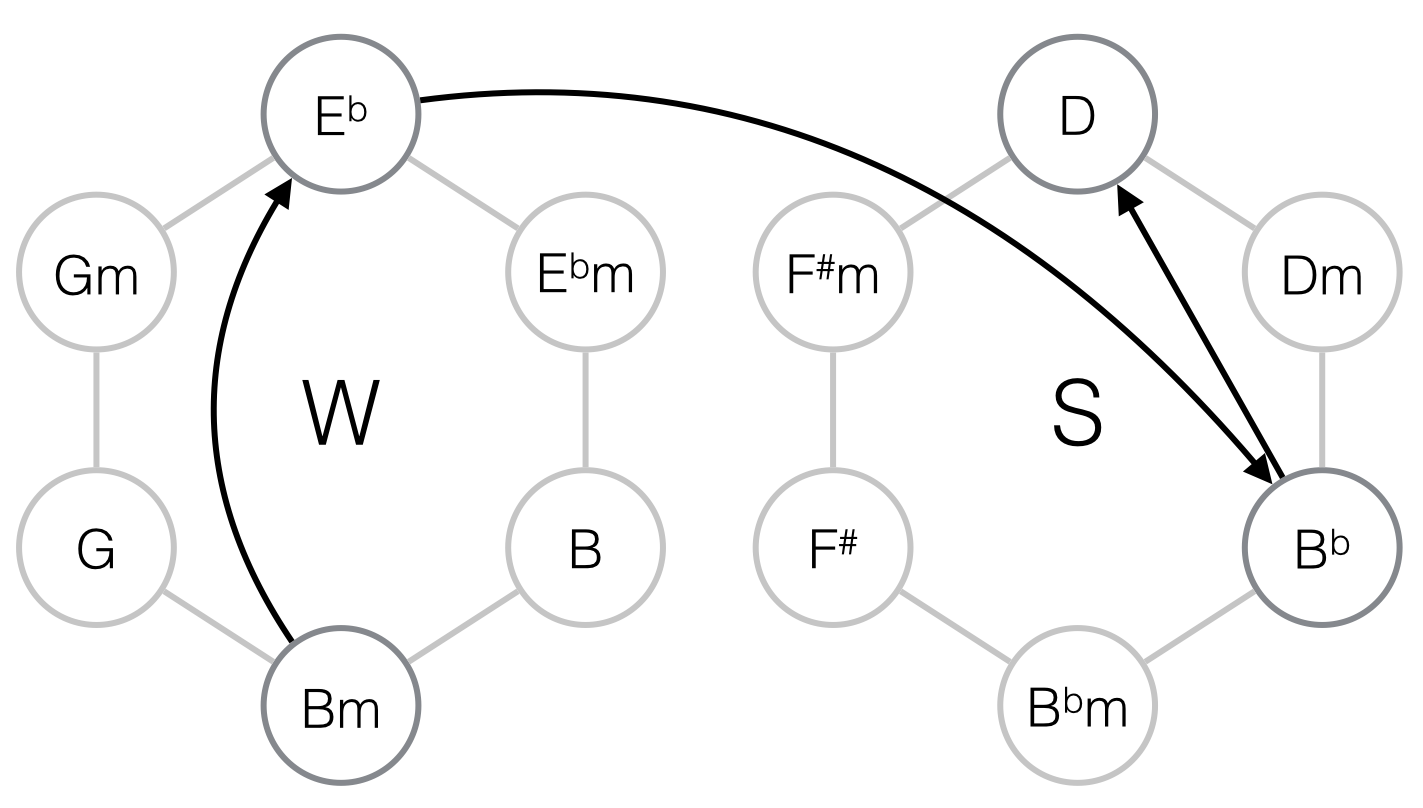
\includegraphics[width=\linewidth]{STTMP_Main_Title_B'''}
	\caption{ST:TMP: Main Title B'' cadence}
	\label{fg:sttmp_main_title_b''_cadence}
	\setfloatalignment{b}
\end{figure}

The four bars of B''' has a solid C pedal over D and the tonality is clearly lydian. The modulation in m.31-32 is possible to view in the \textbf{PL} structures, see figure \ref{fg:sttmp_main_title_b''_cadence}. 

%-----------------------------------------------------------------------------
% A'''
%-----------------------------------------------------------------------------
The final A''' works over a mixolydian G pedal and finishes with a \textit{Aeolian Cadence}, \(\flat{VI}-\flat{VII}\). Overall, the tonality is traceable through the octatonic circles and figure \ref{STTMP_tonal_overview} gives a summary of this.

\clearpage
\begin{figure}
\center
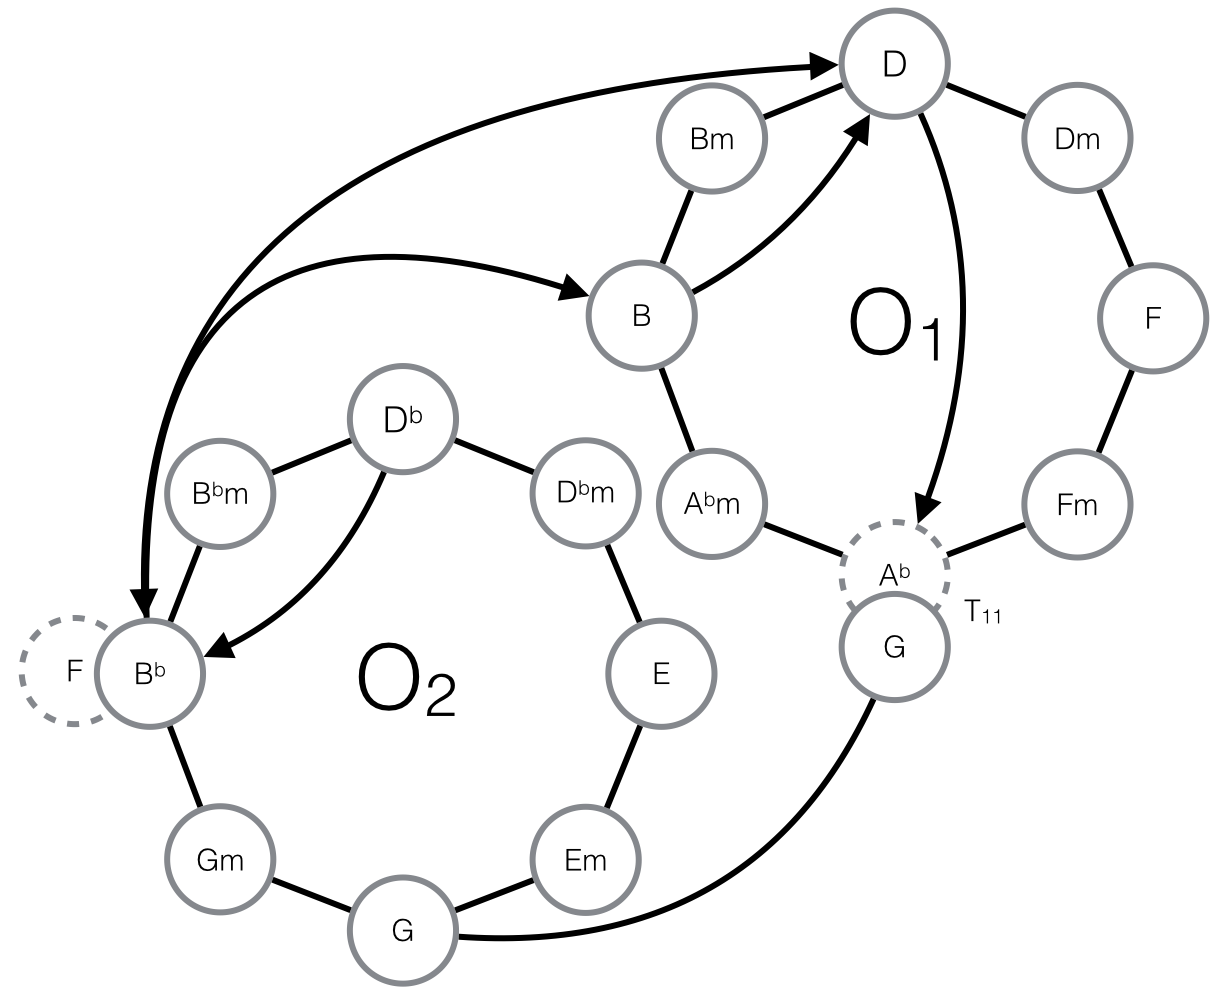
\includegraphics[width=\linewidth]{STTMP_tonal_overview}
	\caption{ST:TMP: Tonal overview}
	\label{STTMP_tonal_overview}
	%\setfloatalignment{b}
\end{figure}


%-----------------------------------------------------------------------------
% PDF
%-----------------------------------------------------------------------------
\clearpage
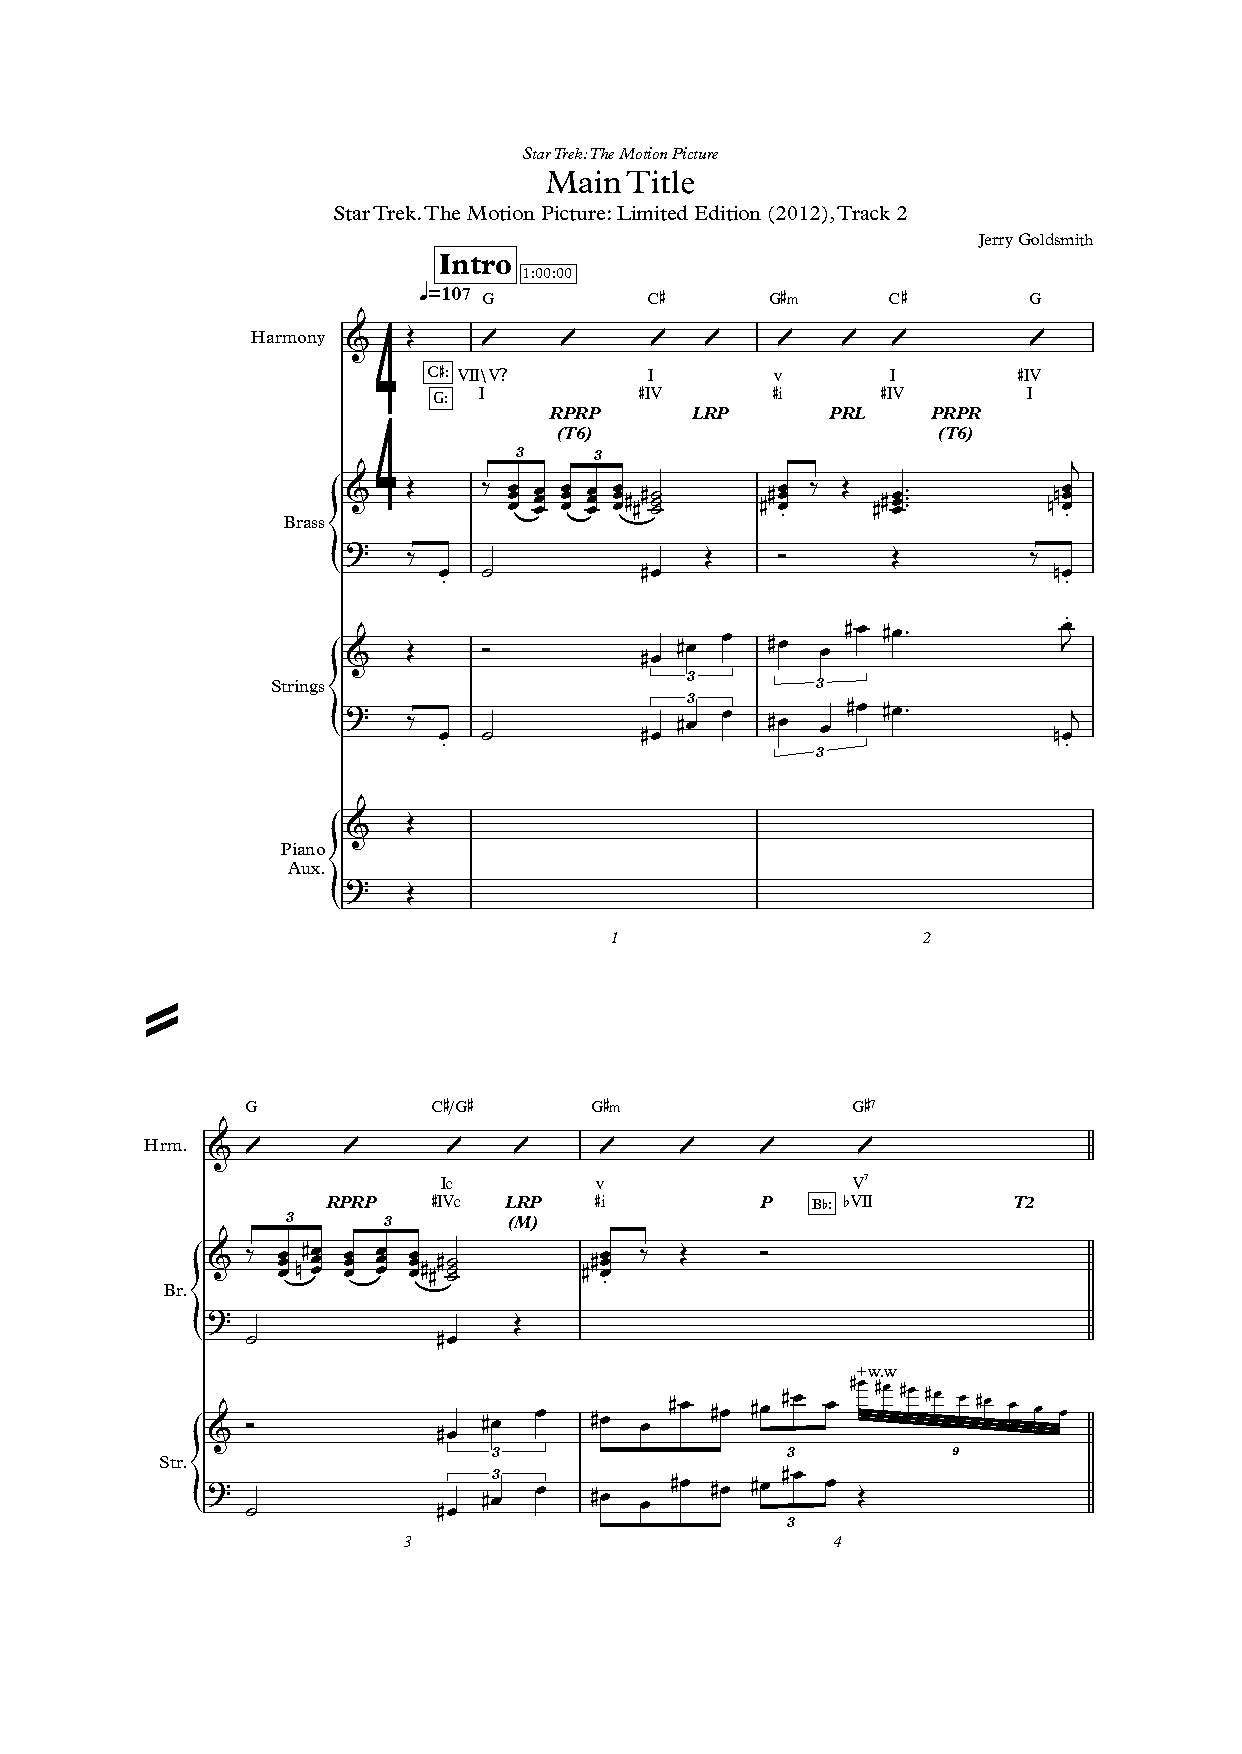
\includepdf[pages=-,pagecommand=\thispagestyle{fancy}]{pdf/st1/STTMP_Main_Title.pdf}

% Reviewed